\section{Taxonomía de Bloom}

La Taxonomía de Bloom inicial, publicada en 1956, fue un sistema diseñado para clasificar los objetivos educativos en niveles de complejidad creciente. Liderada por Benjamín Bloom y un comité de expertos, esta taxonomía se centró originalmente en el dominio cognitivo, estableciendo que el aprendizaje en niveles superiores depende de haber dominado los niveles inferiores.
La estructura original de 1956 se organiza en seis categorías jerárquicas, presentadas mediante sustantivos \cite{bloom1956} de la siguiente manera:
\begin{itemize}
    \item Conocimiento: Se refiere a la capacidad de recordar y reconocer información, hechos específicos, fechas, lugares o términos en la misma forma en que se aprendieron.
    \item Comprensión: Implica entender el significado de la información, ser capaz de interpretarla, resumirla o trasladar el conocimiento a nuevos contextos.
    \item Aplicación: Consiste en hacer uso de la información, métodos o teorías en situaciones nuevas y concretas para resolver problemas.
    \item Análisis: Se enfoca en desglosar la información en sus componentes para entender su estructura organizativa, encontrar patrones o reconocer significados ocultos.
    \item Síntesis: Implica la creación de un producto, plan o propuesta nuevos mediante la combinación de partes y elementos para formar un todo coherente.
    \item Evaluación: Es el nivel más alto y consiste en emitir juicios sobre el valor de ideas, métodos o materiales basándose en criterios y estándares específicos
\end{itemize}

 
A lo largo de las décadas, la taxonomía ha experimentado revisiones significativas para adaptarse a nuevos entendimientos de la psicología cognitiva:
La revisión de Anderson y Krathwohl (2001) transformó los sustantivos originales en verbos (por ejemplo, ``Conocimiento'' pasó a ser ``Recordar'') para reflejar una naturaleza más activa del aprendizaje. Además, se intercambiaron los niveles superiores: Crear pasó a ser la cúspide, mientras que Evaluar se situó en el quinto nivel \cite{anderson2001}. 

\begin{figure}[h]
\caption{Versión revisada por Anderson y Krathwohl, 2001 \cite{uoc2023}}
\centering
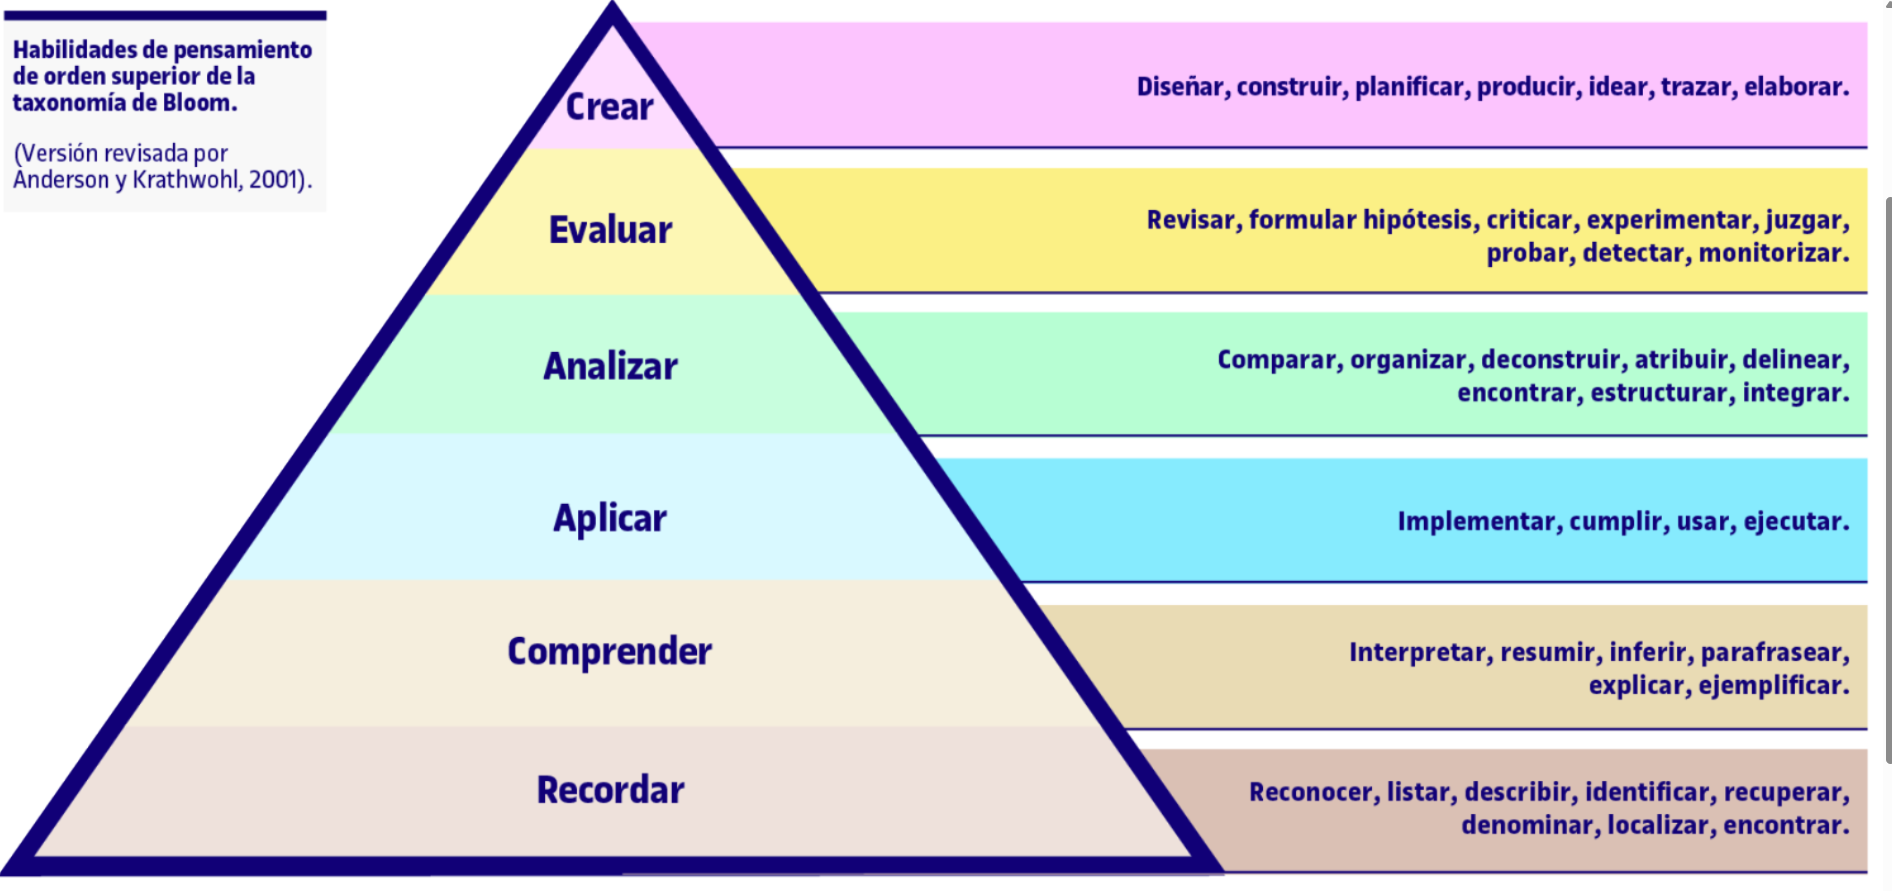
\includegraphics[width=9cm, height=6cm] {imagenes/bloom_2001.png}
\label{bloom_2001}
\end{figure}

En el 2008, Andrew Churches \cite{churches2008} le dio un enfoque a la Taxonomía de Bloom para la Era Digital, esta actualización incorporó verbos y acciones específicas del entorno digital, como ``googlear", etiquetar, piratear, hacer un blog, publicar y compartir, reconociendo que las herramientas tecnológicas potencian cada nivel de pensamiento.

\begin{figure}[h]
\caption{Actualización de la era digital por Andrew Churches, 2008 \cite{uoc2023}}
\centering
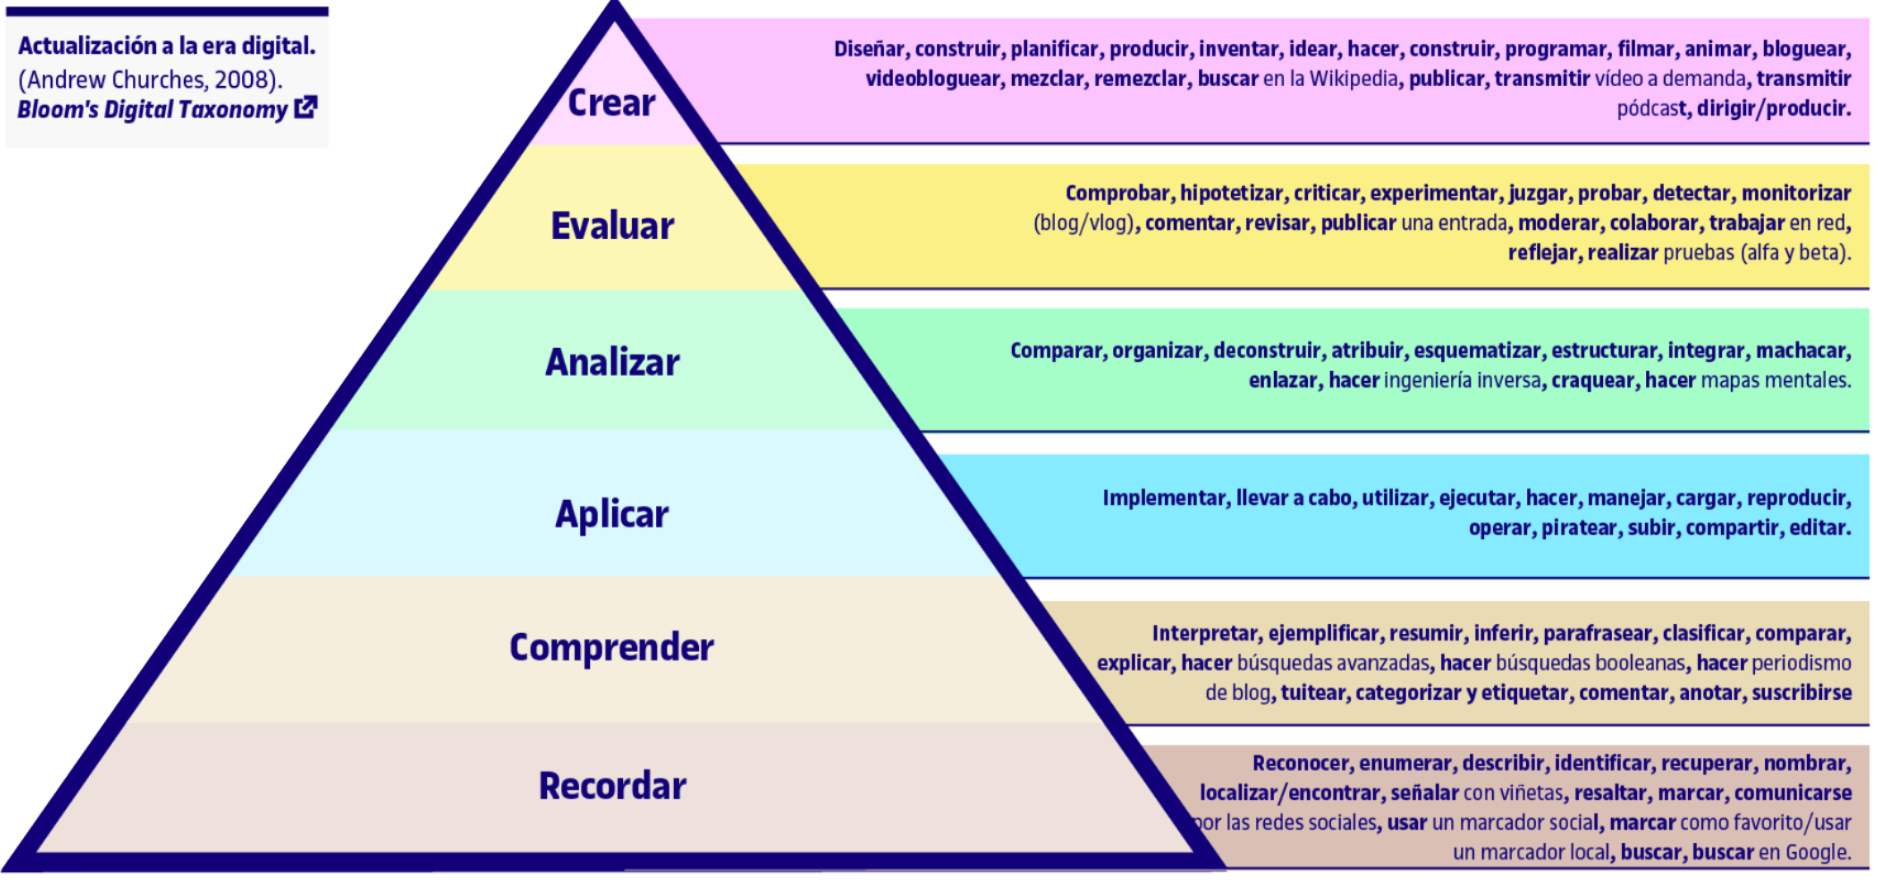
\includegraphics[width=9cm, height=6cm] {imagenes/boom_2008.png}
\label{bloom_2008}
\end{figure}

Las tecnologías digitales interactivas motivaron a Andrew Churches en 2008 a crear la primera adaptación tecnológica significativa de la taxonomía de Bloom donde reconoció que la tecnología no solo proporcionaba nuevas herramientas, sino que estaba transformando fundamentalmente los procesos de aprendizaje, creación y evaluación, anticipando la necesidad de competencias digitales como elementos centrales de la educación moderna.

La revolución de la inteligencia artificial generativa ha catalizado la más reciente y quizás más radical reinterpretación de la taxonomía de Bloom, propuesta por eLearning Innovation Center UOC en 2023, que redefine las habilidades humanas haciendo uso de la IA generativa \cite{uoc2023}. Esta nueva versión representa un cambio desde el uso de herramientas tecnológicas hacia la colaboración entre humanos e inteligencia artificial, donde competencias como el ``prompting'', la detección de alucinaciones y la co-creación estratégica de herramientas y estrategias se convierten en elementos centrales del proceso de generación de conocimiento.\\

\begin{figure}[h]
\caption{Habilidades humanas haciendo uso de la IA generativa por eLinC UOC, 2023 \cite{uoc2023}}
\centering
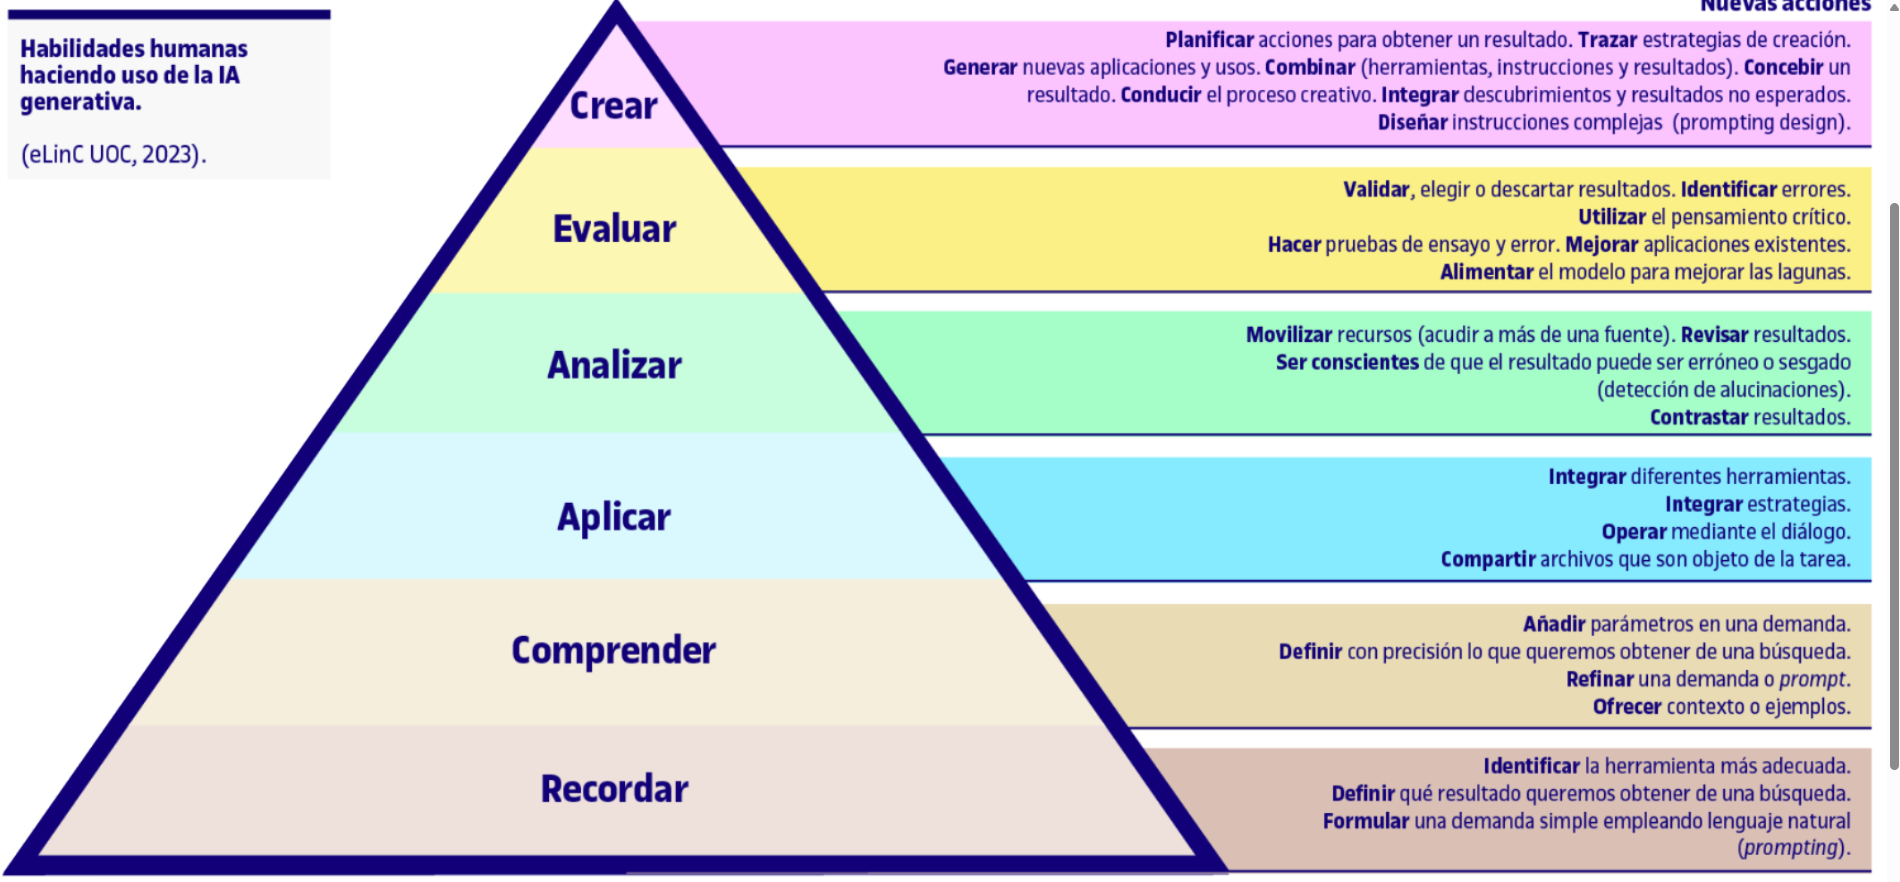
\includegraphics[width=9cm, height=6cm] {imagenes/boom_2023.png}
\label{bloom_2023}
\end{figure}

 La propuesta  reconoce que en un mundo donde la IA puede generar contenido, analizar datos y resolver problemas complejos, el valor humano reside en la capacidad de orquestar estas tecnologías y validar críticamente sus resultados. En este nuevo escenario, el aprendizaje deja de ser un acto puramente individual para convertirse en un proceso donde la tecnología y el razonamiento humano trabajan juntos.